\documentclass{standalone}
\usepackage{graphicx}	
\usepackage{amssymb, amsmath}
\usepackage{color}

\usepackage{tikz}
\usetikzlibrary{intersections, backgrounds, math}
\usepackage{pgfmath}

\definecolor{light}{RGB}{220, 188, 188}
\definecolor{mid}{RGB}{185, 124, 124}
\definecolor{dark}{RGB}{143, 39, 39}
\definecolor{highlight}{RGB}{180, 31, 180}
\definecolor{gray10}{gray}{0.1}
\definecolor{gray20}{gray}{0.2}
\definecolor{gray30}{gray}{0.3}
\definecolor{gray40}{gray}{0.4}
\definecolor{gray60}{gray}{0.6}
\definecolor{gray70}{gray}{0.7}
\definecolor{gray80}{gray}{0.8}
\definecolor{gray90}{gray}{0.9}
\definecolor{gray95}{gray}{0.95}


\begin{document}

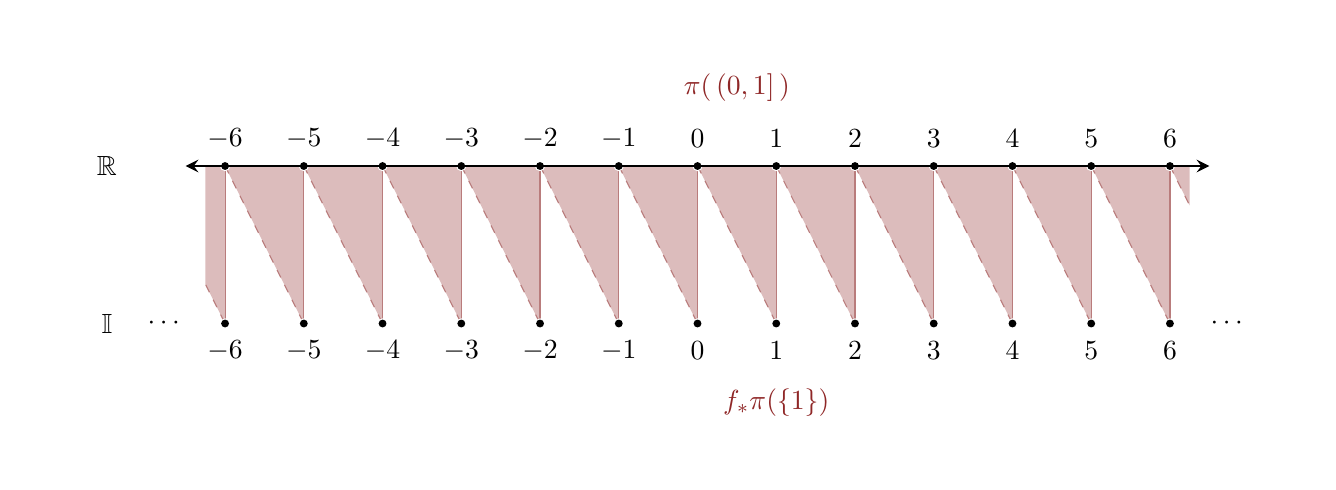
\begin{tikzpicture}[scale=1]
  \begin{scope}[shift={(0, 0)}]
    \draw[white] (-8.5, -5.75) rectangle (7.75, -0.25);
    
    \begin{scope}
      \clip (-6.25, -2) rectangle (6.25, -4);
      \foreach \n in {-7, -6, ..., 6} {
        \pgfmathsetmacro{\x}{\n};
        
        \fill[light] (\x, -2) -- (\x + 1, -2) -- (\x + 1, -4) -- cycle;
        \draw[mid, dashed] (\x, -2) -- (\x + 1, -4);
        \draw[mid] (\x + 1, -2) -- (\x + 1, -4);
      }
    \end{scope}
    
    \foreach \n in {-6, -5, ..., 6} {
      \pgfmathsetmacro{\x}{\n};
      
      \fill[white] (\x, -4) circle (0.065);
      \fill[black] (\x, -4) circle (0.05);
      \node at (\x, -4.35) { $\n$ };
      
      \fill[white] (\x, -2) circle (0.065);
      \fill[black] (\x, -2) circle (0.05);
      \node at (\x, -1.65) { $\n$ };
    }
    
    \draw[<->, >=stealth, line width=1] (-6.5, -2) -- (6.5, -2);
 
    \node at (-7.5, -4) { $\mathbb{I}$ };
    \node at (-7.5, -2) { $\mathbb{R}$ };

    \node at (+6.75, -4) { $\cdots$ };
    \node at (-6.75, -4) { $\cdots$ };
    
    \node[dark] at (0.5, -1) { $\pi ( \, (0,  1 ] \, )$ };
    \node[dark] at (1, -5) { $f_{*} \pi ( \{ 1 \} )$ };
  \end{scope}
  
\end{tikzpicture}

\end{document}  